\chapter{Introduction}

Internet has become another world itself in which you can get everything which is sufficient to live a life. You can watch movie, order food, earn money make friends and find your soul mate even. It has created huge revolution in our life. According to statics, almost 3 billion users have access of internet. Unfortunately, this world has become very vulnerable and unsafe. Internet banking, ecommerce, email services share significant amount of usage of this modern world. Often information and data being transmitted through the internet is very valuable and confidential. Poor security and some vulnerabilities have made easy to gain access of such confidential data for bad programmers. 

Among all of these security attacks, Phishing attack is known for stealing private information. According to Kaspersky Lab’s database, 1 million number of phishing attacks has been increased in the first quarter of 2015 compare to previous quarter.  World is becoming online which has increased the number of websites so as phishing attacks. Phishing attacks indirectly affect many well know organization’s reputation. Many solutions were provided till now to detect phishing websites. None of those solutions provides good accuracy and performance when it comes real time safe browsing. 


\section{What is phishing} 

Phishing can be defined as activity of collecting unauthorized and confidential data such as username, password, credit card detail, bank account details electronically. First time phishing activity was defined in detail in a paper and presentation delivered to the 1987 International HP Users Group, Interex [2]. First phishing attack was registered by AOHell hacking tool [3]. 

There are various types of phishing attacks. Phishing can be done in numerous ways. Following is the type of phishing attacks.

\begin{itemize}
\item Link manipulation
\item Filter evasion
\item Website forgery
\item Covert redirect
\item Phone phishing
\end{itemize}

Our main focus in on “Link manipulation” type of phishing attack. In this attack URLs appear to belong to the valid organization. URLs are obfuscated very smartly that it is difficult sometimes to differentiate by human eye also. Let’s take an example of such website. 

As you can see in the first image this site claims to be genuine Paypal, a worldwide online payments system company. Second image is the real original website of Paypal. If you closely look then you easily see the difference between two websites. There are some visible difference between these two websites like logo of the company, favicon and secured certificate. Different types of techniques is used to redirect such fake websites. Sometimes users do not see this visible difference and becomes the victims of this phishing attacks. 

Once the data is collected, different types of forgeries is done by hackers. This scam can be of Millions of money sometimes. Sometimes its all about private and confidential information of celebrity which can be leaked to spoil the image of the same person.  

\begin{figure}[htb]
\centering
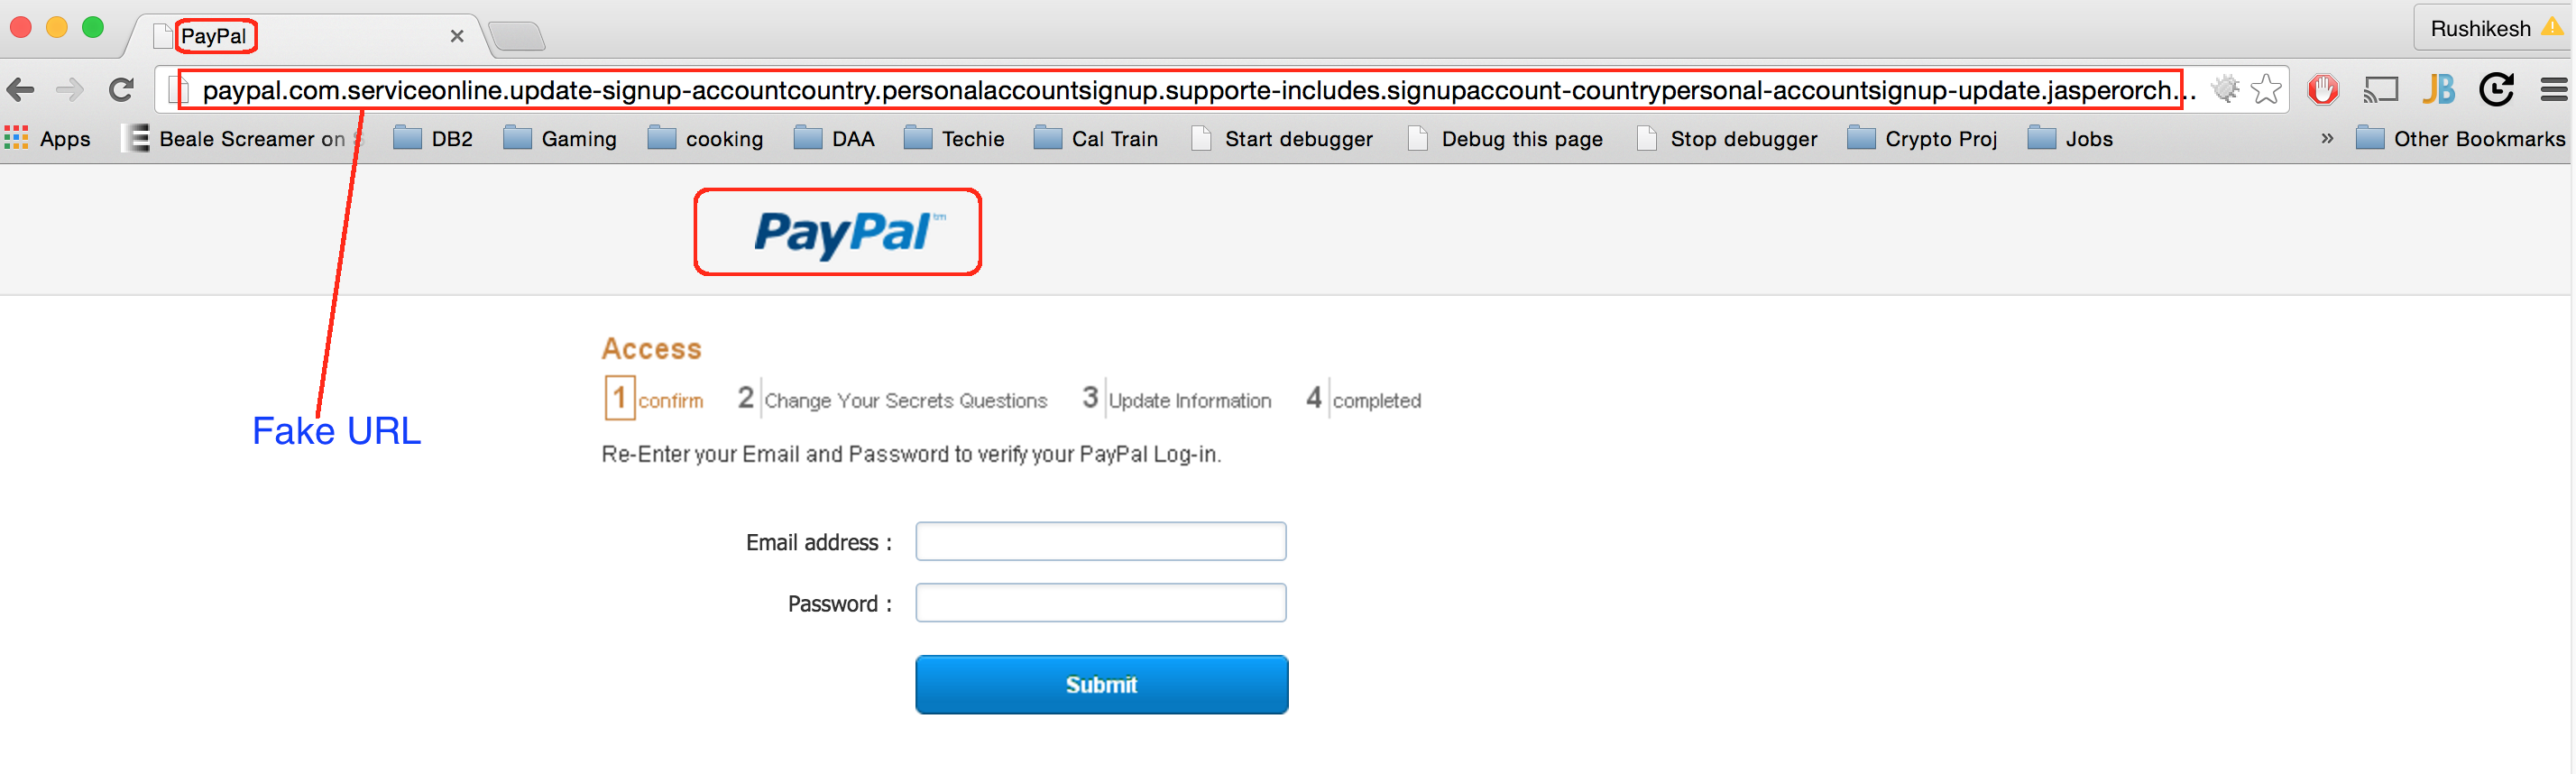
\includegraphics[width=0.9\textwidth]{images/Paypal_fake_site.png}
\caption{Fake Paypal website} 
\label{fig:fake_paypal_website}
\end{figure}



\begin{figure}[htb]
\centering
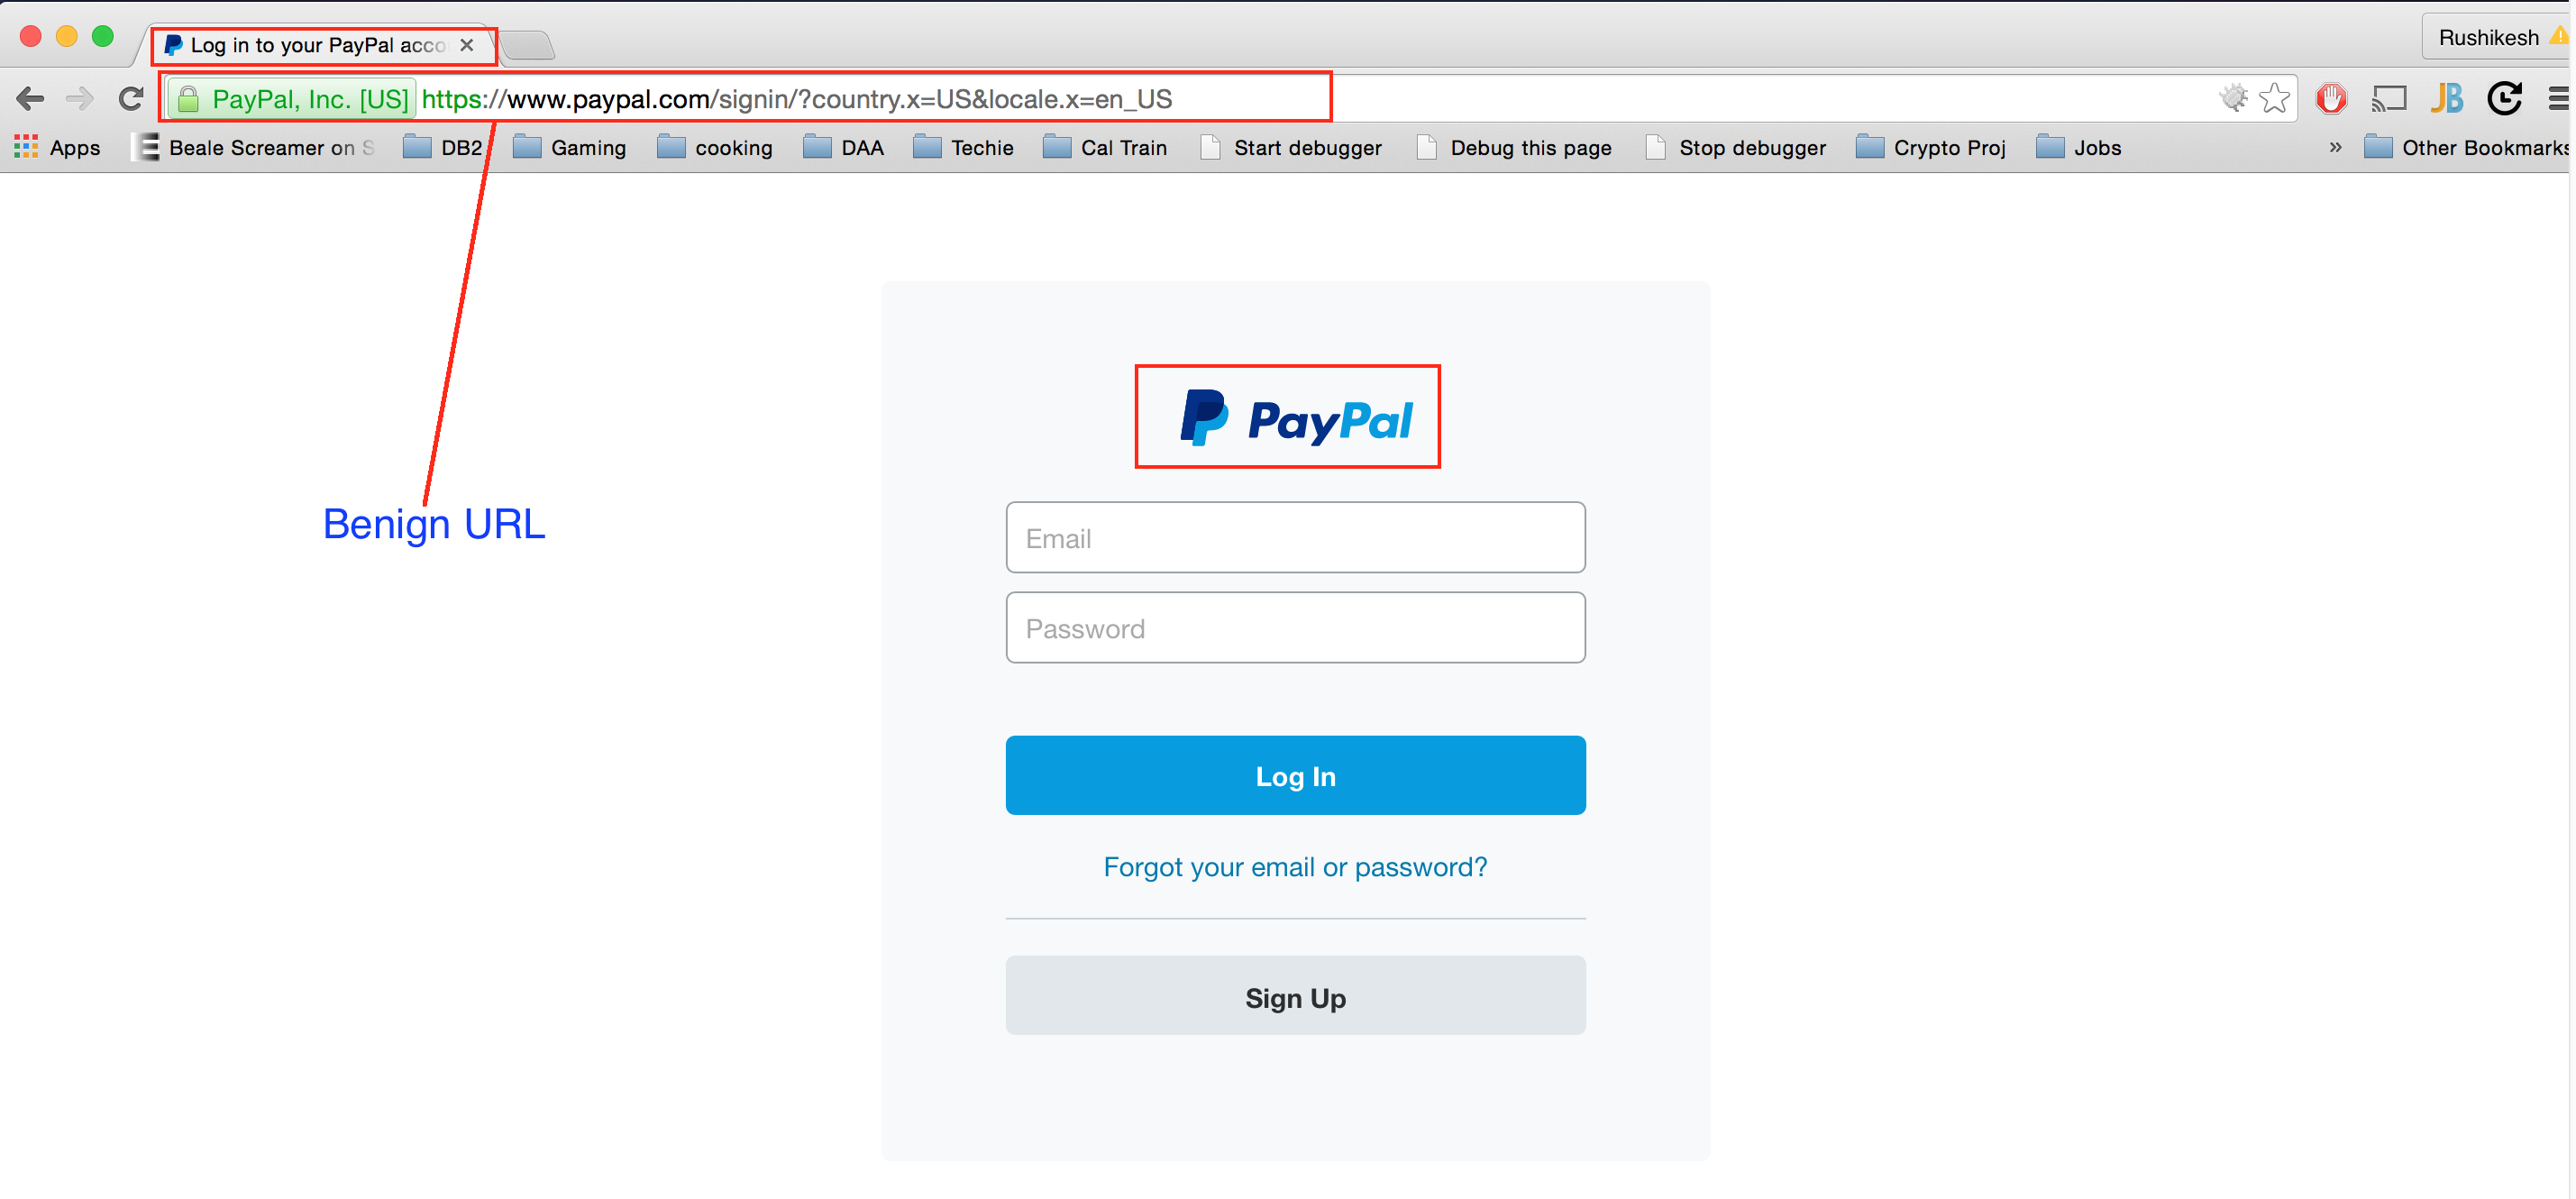
\includegraphics[width=0.9\textwidth]{images/Paypal_original_site.png}
\caption{Original Paypal website} 
\label{fig:original_paypal_website}
\end{figure}



\section{Problems}

To address this Phishing problems lots of academic and business research has been done so far. These methods either uses blacklist methods or some type of heuristics or machine learning techniques. Blacklist method is more common and popular for all the browser. All browser contains some manually verified list of phishing websites. This technique contains fairly low positive rate. But when it comes to fresh phishing website, it does fail. It is not much effective to newly developed phishing websites.

Second approach is to adopt smart heuristics which is given some training data to train the heuristic. This heuristic collects different types of features of the websites and based on that it decides the authenticity of the website. So far no heuristic has defined which has better accuracy, performance and seamlessly browsing experience. In addition, scope of the detection of phishing website should not be limited. We referred to similar kind of one research paper which talks about all of these features. We tried to collect all the mentioned attributes and experimented with different machine learning classifiers. This method highly depends on approximate string matching algorithms and WHOIS server queries. In the development procedure we used only one third party services which is WHOIS server. Otherwise every algorithm run on native system. Our tests with this method shows some promising results. With the help of this attributes and approach we were able to achieve almost 97% accuracy and comparatively good performance with respect to time.

One more research paper has proposed to use image processing techniques. They tried to emphasize on the favicon of the website. They proved that significant difference is found when you compare the favicon of original website and spoofed website. Limitation of this approach is website must have favicon otherwise this method will fail. 


\section{My contribution}

My main role was go give practical shape to the idea which they talked in the research paper. Since everything was on the paper only and they did not talk about any implementation part, it required lot of efforts to make it practical. 

There are couple of different way to make things happens. We split this entire addons in three different parts. First component resides on client side. Second component is web services which is kind of middle layer between third component, machine learning algorithms and addons. 

We opted for making firefox addons. It has got pretty nice documentation to start with. Then there were couple of options available for machine learning libraries. Weka seemed quite distant options for us. It provides api for different languages.

We collected different samples of phishing websites from Phishtank[] which is famous organization for providing database of phishing websites. We used Alexa to get samples of benign websites. Total 1773 URLs collected for training data set. Out of 1773 URLs 829 URLs were phishing and 944 URLs were benign. We tried to apply different machine learning classifiers to get the best accuracy. As per our results, our filter achieves almost 97% accuracy to detect phishing websites. 


